\section{Discussion and limitations}
The main limitation of the rainfall comparison is the changing station
network. No station met the 90\% annual-coverage rule in every year, so the
across-year results should not be interpreted as a fixed-network climate trend.
For prediction, all 2024 stations were already present in the training period,
so transfer to new stations was not tested. The archive also does not record
when corrected observations became available, which prevents us from
verifying that every feature would have been available in real time.

Results from 2024 had been inspected during an earlier development iteration.
The reported model was subsequently fixed using only pre-2024 data, but 2024
should therefore be treated as the final evaluation period rather than a
completely untouched test set. On this period, PR-AUC and Brier score improved
over climatology at all six thresholds, while weighted ECE remained slightly
higher. Predictions require a valid current observation, and labels require
all six future readings.

\section{Conclusion}
Rainfall occurrence varied substantially across 2017--2024, with a consistent
afternoon peak but no fixed station cohort available for direct long-term
comparison. For prediction, adding same-station rainfall history increased
GBT mean PR-AUC on the 2022 selection sample from 0.03553 to 0.52207. On the
2024 evaluation period, the final model achieved PR-AUC 0.6345 and Brier score
0.01958 at 0.5~mm, compared with 0.0732 and 0.03436 for climatology. Isotonic
calibration reduced aggregate calibration error, and PAVA removed the
remaining cross-threshold monotonicity violations.

\section*{AI use declaration}
\addcontentsline{toc}{section}{AI use declaration}
GPT-6 was used for coding assistance, debugging and language editing. The
authors ran the experiments and checked the reported results.

\clearpage
\addcontentsline{toc}{section}{References}
\begin{thebibliography}{9}
\small
\raggedright
\setlength{\itemsep}{0pt}
\bibitem{nea}
National Environment Agency. \emph{Historical Rainfall across Singapore}.
data.gov.sg. \url{https://data.gov.sg/collections/2279/view}.

\bibitem{spark}
Apache Spark. \emph{Spark 3.5.3 Release Notes}.
\url{https://spark.apache.org/releases/spark-release-3-5-3.html}.

\bibitem{mllib}
Apache Spark. \emph{Extracting, transforming and selecting features}, Spark
3.5.3 documentation. \url{https://spark.apache.org/docs/3.5.3/ml-features.html}.

\bibitem{dataprocimage}
Google Cloud. \emph{2.2.x release image versions}.
\url{https://docs.cloud.google.com/managed-spark/docs/concepts/versioning/image-release-2.2}.

\bibitem{gceE2}
Google Cloud. \emph{General-purpose machine family for Compute Engine}.
\url{https://docs.cloud.google.com/compute/docs/general-purpose-machines}.

\bibitem{sklearnroc}
Scikit-learn Developers. \emph{roc\_auc\_score}.
\url{https://scikit-learn.org/stable/modules/generated/sklearn.metrics.roc_auc_score.html}.

\bibitem{sklearnpr}
Scikit-learn Developers. \emph{precision\_recall\_curve}.
\url{https://scikit-learn.org/stable/modules/generated/sklearn.metrics.precision_recall_curve.html}.
\end{thebibliography}

\clearpage
\appendix
\setcounter{figure}{0}
\renewcommand{\thefigure}{\Alph{figure}}
\begin{landscape}
\thispagestyle{plain}
\section{Spark UI evidence}
The figures are saved Spark History Server views from the final GBT-B
application on the eight-worker cluster. Executor totals are the completed
application's recorded values; worker labels are anonymised.
\begin{center}
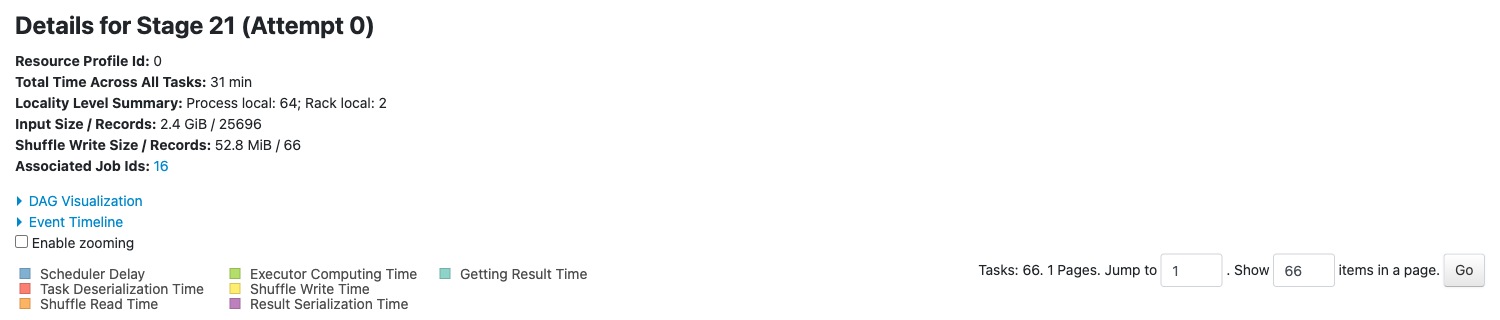
\includegraphics[width=0.95\linewidth]{figures/final/spark_ui_final_stage.png}
\captionof{figure}{Spark History Server detail for Stage 21 of the final GBT-B
application. The imputation-statistic stage completed 66 tasks, reading
2.4~GiB and writing 52.8~MiB of shuffle data.}
\label{fig:spark-ui-final-stage}
\end{center}
\end{landscape}

\clearpage
\begin{landscape}
\thispagestyle{plain}
\begin{center}
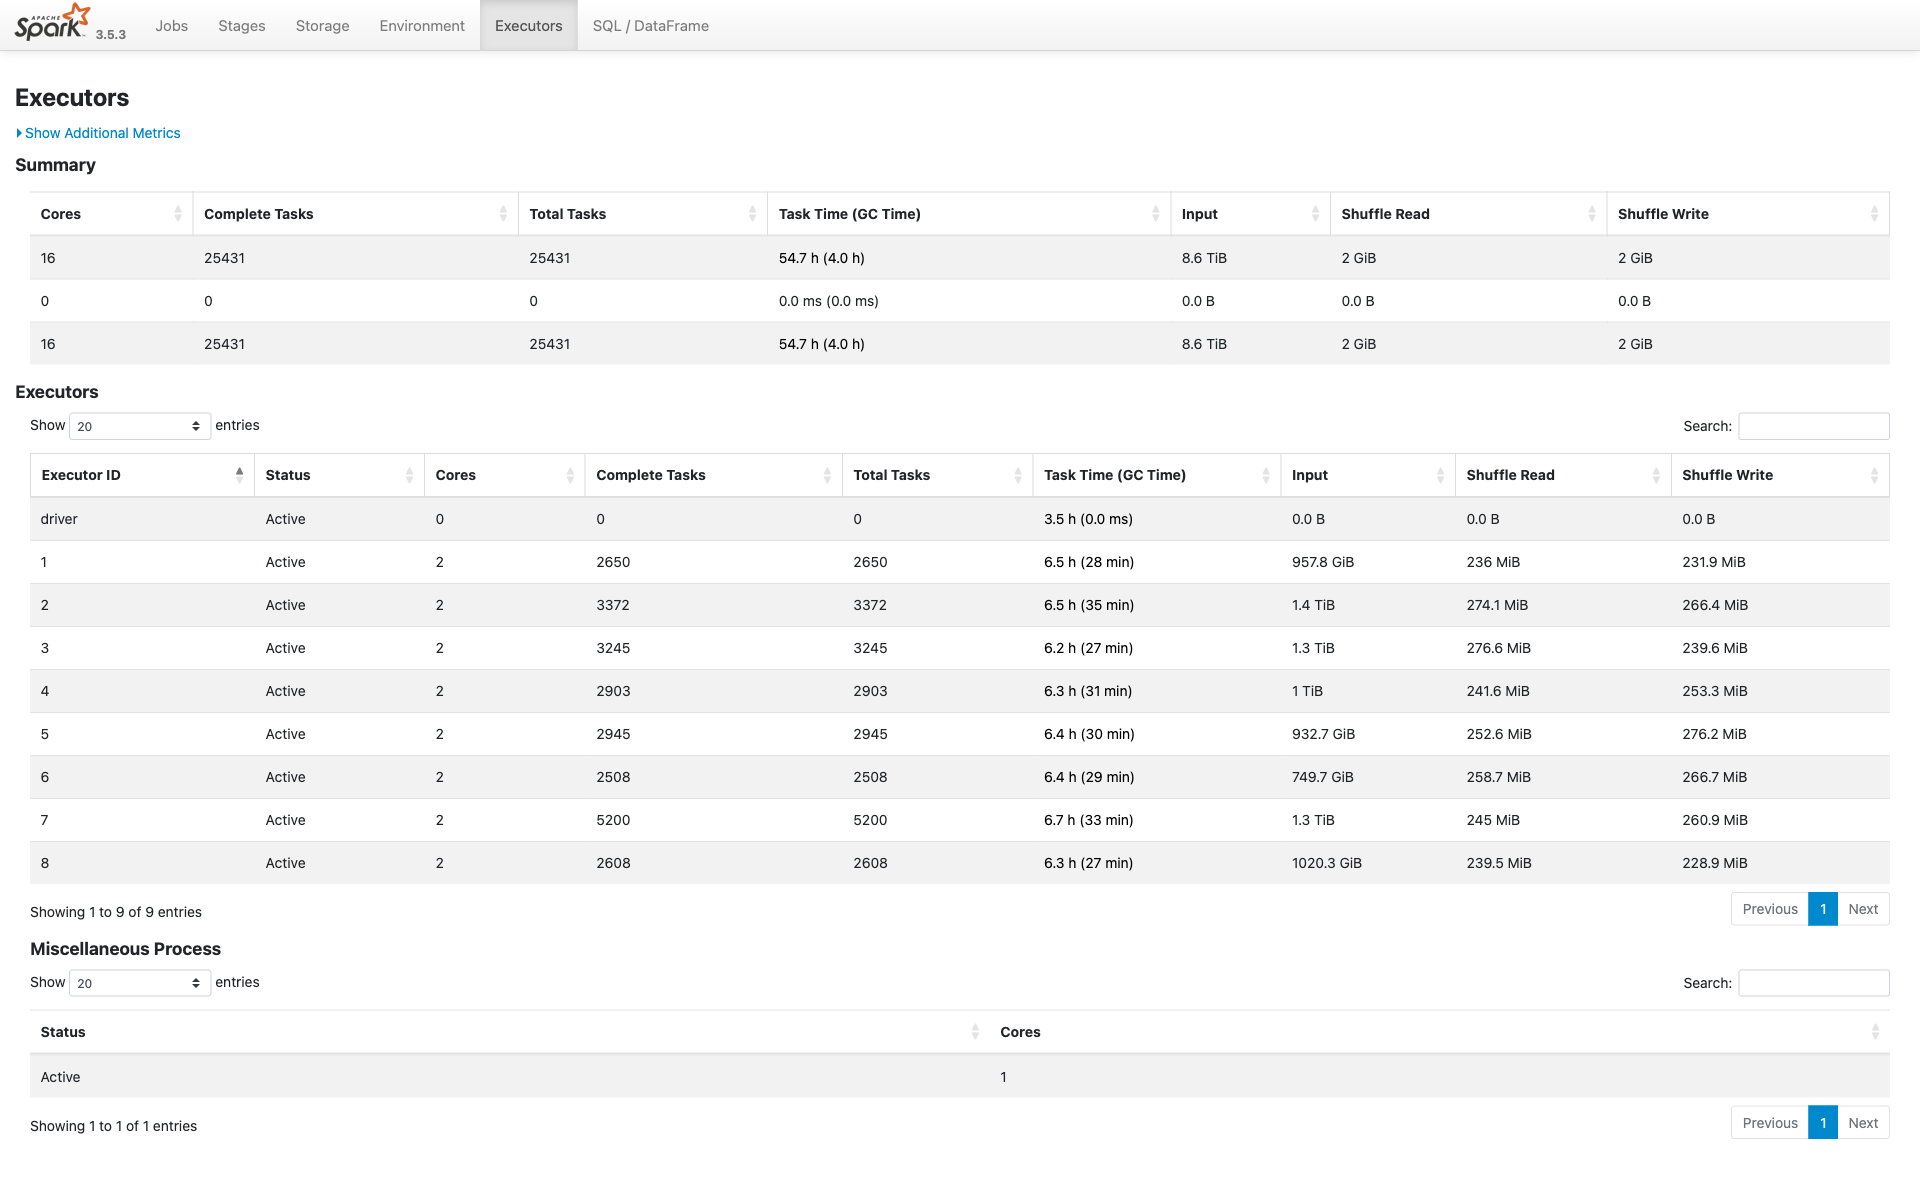
\includegraphics[width=0.92\linewidth]{figures/final/spark_ui_final_executors.png}
\captionof{figure}{Executors view for the same final GBT-B application. Spark
lists the driver and eight worker executors; the workers supplied 16 cores and
completed 25,431 tasks. Application totals were 8.6~TiB input, 2~GiB shuffle
read and 2~GiB shuffle write; worker labels are anonymised.}
\label{fig:spark-ui-executors}
\end{center}
\end{landscape}

\end{document}
